\chapter{Genetické programování}

\section{Základní princip}
Genetické programování je evoluční technika, která vytváří počítačové programy. Cílem genetického programování je vyřešit co nejlépe zadaný problém.
Nespecifikujeme jak je potřeba ho vyřešit, ale víme, co je potřeba vyřešit.
\par
Každý program budeme nazývat jedincem a množině jedinců budeme říkat populace. Algoritmus pak běží iterativně v generacích. 
V každé iteraci se provede výběr nějakých jedinců z populace, ti se pomocí genetických operátorů upraví a nakonec se rozhoduje, kteří z nich přežijí do další generace.
Populaci na začátku iterace nazýváme rodiče a populaci, která bylo nakonci iterace pro další generaci, nazýváme potomky.
Každý program představuje jedno řešení daného problému. Kvalitu tohoto řešení ohodnocujeme takzvanou fitness funkcí. Čím vyšší hodnotu této funkce jedinec získá, tím lépe řeší daný problém.
\subsection{Reprezentace}

Program je obvykle reprezentovaný syntaktickým stromem. Stromy ve vnitřních uzlech obsahují funkce (neterminály) a v listech terminály.
Vyhodnocení stromu probíhá od listů ke kořeni a výsledek programu je pak hodnota kořenu.

\subsection{Inicializace populace}
Na začátku evoluce potřebujeme inicializovat populaci. Na počátku jsou jedinci vytvořeni náhodně. Obvykle se k vytvoření jedinců používají dvě metody.
První z nich je vytváření jedinců s pevně danou hloubkou stromu, kde v listech jsou vždy už jen terminály. Druhou metodou je stavět strom náhodně z předem daného počtu neterminálů.
Po vyčerpání počtu neterminálů se již opět přidají terminály jako listy. Tato metoda vytváří jedince různých velikostí a tvarů.
Častou praxí je prvotní populaci vytvořit tak, že každá z metod vytvoří polovinu jedinců. 

\subsection{Selekce}
V každé iteraci chceme vybrat několik jedinců, nad kterými budeme provádět různé genetické operátory. Snahou je vybírat jedince s vyšší hodnotou fitness funkce.
Asi nejpoužívanější metodou selekce je turnajová selekce. Náhodně se zvolí daný počet jedinců, ti se porovnají mezi sebou na základě jejich hodnoty fitness funkce a nejlepší z nich je pak zvolen do výběru.
Dalším z mnoha metod selekce je ruletová selekce. Zde je pravděpodobnost zvolení jedince do výběru přímo úměrná jeho hodnotě fitness funkce.
Pravděpodobnost výběru i-tého jedince je 
\newline $p(i) = \frac{f(i)}{\sum_{j=1}^{n} f(j)} $. \newline
Ruletová selekce má jednoduchou implementaci a zároveň je rychlá na výpočet. 
Jejím problémem je ale předčasná konvergence k lokálnímu optimu.
\par
Genetické operátory mohou občas upravit nejlepšího jedince tak, že se jeho hodnota fitness funkce výrazně zhorší.
Z tohoto důvodu se často používá technika zvaná elitismus, která automaticky do další generace vybere několik nejlepších současných jedinců. 
Tímto způsobem máme zajištěno, že neztratíme nejlepší jedince.



\url{https://www.researchgate.net/publication/259461147_Selection_Methods_for_Genetic_Algorithms}

\subsection{Genetické operátory}
Genetické operátory jsou dvojího druhu, křížení a mutace. Myšlenkou křížení je vzít dva jedince, nazývejme je rodiče, a pomocí křížení informací každého z nich vytvořit nového potomka.
V genetickém programování pracujeme s jedinci reprezentovanými stromy, proto křížení jedinců představuje křížení jejich stromů. V každém z rodičů se zvolí jeden uzel. 
Výsledný potomek vypadá jako první rodič, jen na původním místě vybraného uzlu bude nyní podstrom, který je zavěšený pod vybraným uzlem druhého rodiče.
\par
Druhým genetickým operátorem je mutace, ta již nepotřebuje mít dva rodiče, ale úprava se provede nad jedincem samotným.
Mutovat můžeme v jedinci buď jediný bod, nebo celý nějaký podstrom. V případě mutace podstromu se namísto vybraného podstromu vygeneruje zcela nový podstrom. 
Toto v zásadě představuje křížení s novým náhodně vytvořeným jedincem.
\newline
Mutace jediného bodu změní náhodně jediný uzel ve stromě. V případě terminálu se může vybrat libovolný jiný terminál. A v případě vnitřního uzlu může být vybraný libovolný jiný neterminál, který je stejné arity.

\subsection{Silně a volně typované genetické programování}
Ve volně typovaném genetickém programování nezadáváme typy funkcí ani terminálů. Jediné co musíme u funkcí určit je jejich arita a na základě toho se generují a mutují jedinci korektně.
Obvykle se nám více bude hodit silně typované genetické programování, zde určujeme u všech funkcí nejen jejich aritu, ale také typ každého z argumentů dané funkce a také typ návratové hodnoty.
Podobně musíme určit i hodnotové typy terminálů. Díky tomu máme zaručeno, že pokud máme například funkci, která vrací typ boolean, tak tato hodnota nebude vynásobena hodnotou typu float. 
Pak jen určíme hodnotové typy celého problému a algoritmus už se postará o to, aby byly typové podmínky dodrženy.
\url{https://deap.readthedocs.io/en/master/tutorials/advanced/gp.html}

\section{Využití}
Genetické programování je využitelné ve všech problémech, kde jsme schopní vymyslet způsob jak reprezentovat jedince představujícího řešení problému a fitness funkci, díky které jsme schopni dané řešení ohodnotit.
To tedy znamená, že možnosti využití jsou téměř nekonečné. Zmiňme ale pár konkrétních příkladů. 

\subsection{Obecné využití}
\todo{volně přeloženo a zkráceno z původního textu str. 126}
Obecně se genetické programování ukazuje být vhodné ve všech problémech, které splňují některou, z následujících podmínek:

\begin{itemize}
    \item Vzájemné vztahy zkoumaných proměnných nejsou dobře známy, nebo je podezření, že jejich současné porozumění může být mylné.
    \item Nalezení velikosti a tvaru hledaného řešení je částí řešeného problému.
    \item Existují simulátory pro testování vhodnosti zadaného řešení, ale neexistují metody pro přímé získání dobrých řešení.
    \item Obvyklé metody matematické analýzy nedávají, nebo ani nemohou být použity pro získání analytického řešení.
    \item Přibližné řešení je zcela postačující.
    
\end{itemize}

\subsection{Symbolická regrese}
V mnoha problémech je naším cílem nalézt funkci, jejíž hodnota splňuje nějakou požadovanou vlastnost. Toto známe pod názvem symbolická regrese.
Obyčejná regrese má obvykle za cíl nalézt koeficienty předem zadané funkce, tak aby co nejlépe odpovídala daným datům.
Zde je problém, že pokud potřebná funkce nemá stejnou strukturu, jako zadaná funkce, tak dobré koeficienty nenalezneme nikdy a musíme zkusit hledat funkci jiné struktury.
Tento problém může vyřešit právě symbolická regrese. Ta hledá vhodnou funkci aniž by na začátku měla očekávání o její struktuře.
Uvedeme triviální příklad. Řekněme, že hledáme výraz, jehož hodnoty odpovídají polynomu $x^2+x+1$ na intervalu $[-1,1]$.
Budeme hledat funkci jedné proměnné $x$, proto $x$ přidáme jako terminál. Dále přidáme jako terminály číselné konstanty (například -1,1,2,5,10), které budou sloužit pro hledání koeficientů.
Pro náš případ bude stačit, když si jako aritmetické funkce přidáme ty základní, tedy sčítání, odečítání, násobení a dělení.
Fitness funkci můžeme zvolit jako součet absolutních hodnot rozdílů daného výrazu a hledaného výrazu $x^2+x+1$.
Toto stačí pro spuštění evolučního algoritmu. 
V takto triviálním případě se hledané řešení nalezne pravděpodobně vezmi brzo a bude mít jednu z podobu stromu reprezentujícího daný výraz (viz strom výrazu \ref{obr04:GrafFormule})


\begin{figure}[p]\centering
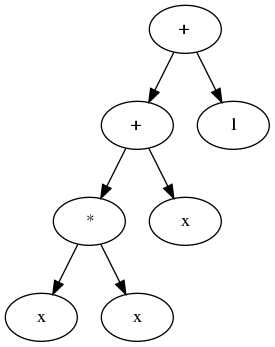
\includegraphics[width=70mm, height=70mm]{./Obrazky/formule_graph_2.png}
\caption{Strom výrazu}
\label{obr04:GrafFormule}
\end{figure}


\subsection{Další příklady použití}
Symbolická regrese je jen jedním z mnoha problémů, které lze řešit pomocí genetického programování.
\todo{Podobě jako ve field guide to genetic programming vyjmenovat konkrétní výsledky s odkazy na stejné články jako v knize? 
Nebo zmínit jen oblasti bez vysvětlování konkrétních problémů? - (Bioinformatika, počítačové hry, Ekonomické modely, Umění)}

\section{Aplikace}
\subsection{Úvod}
Genetické programování lze využít i v mém problému hledání inteligentního agenta. 
Nezbytným požadavkem pro využití genetického programování je existence reprezentace jedince a fitness funkce, která mu přiřadí jeho hodnotu. 
Jedinec bude představovat rozhodovací funkci, která se na základě vstupních argumentů rozhodne, který akční plán bude vybrán.

V našem případě máme hru, kde spolu dva hráči soupeří a hra končí výhrou jednoho z hráčů.
Přesně tohoto můžeme ve fitness funkci jedince využít. 
Pokud chceme využít výsledku hry, jak jedinec ve hře dopadl, tak musíme ale nejprve zvolit proti jakému hráči bude jedinec, který je předmětem našeho zájmu, hrát.

Genetické programování jsem využil ve dvou experimentech. 
Reprezentace jedince je pro oba experimenty stejná, rozdíl je ale v přístupu k fitness funkcím, ty popíšu v každém experimentu separátně.

Pro experimentování s genetickým programováním jsem zvolil knihovnu deap pro python. Zde lze jednoduše konfigurovat evoluční algoritmus na konkrétní řešený problém.
Stačí popsat jak reprezentovat jedince a jaká je jeho fitness funkce a zbytek knihovna vyřeší za nás.


\subsection{Reprezentace jedince}
V předchozí kapitole jsme si vybudovali abstrakace v podobě senzorů a akčních plánů a těch zde budeme chtít využít.
Jedinec, podobně jako u symbolické regrese, je funkce, tedy může být reprezentován stromem.

\begin{itemize}
\item{
    Terminály:
    \begin{itemize}
        \item Vstupní argumenty rozhodovací funkce
        \item Celočíselné konstanty -1, 1, 3, 5, 10, 100
        \item Nulární funkce vracející výčtové hodnoty reprezentující zvolený akční plán  
    \end{itemize}
    Jako argumenty funkce jsem si zvolil následující hodnoty: délky všech čtyř akčních plánů a počet kroků před srážkou vesmírné lodi s asteroidem.
    Délky akčních plánů se pohybují v intervalu $(1,100)$, proto jsou číselné konstanty zvoleny tak, aby se jejich sčítáním a násobením lehce dosáhlo dalších hodnot z tohoto intervalu.
    }

\item{
    Neterminály:
    \begin{itemize}
        \item Aritmetické operace sčítání a násobení
        \item Funkce \emph{compare}
        \item Funkce \emph{if\_then\_else}
    \end{itemize}
    Z aritmetický operací nám stačí sčítání a násobení. Operaci odčítání získáme pomocí sčítání a násobení konstantou -1. 
    Hodnoty z intervalu $(1,100)$ jednoduše získáme také pomocí sčítání a násobení potřebných konstant, proto pro operaci dělení není důvod.
    Všechny aritmetické operace jsou typu $([int,int], int)$.
    Funkce \emph{compare} je typu $([int,int], Bool)$, vrací zda první argument je větší než druhý argument.
    Poslední použitá funkce \emph{if\_then\_else} je typu 
    \newline
    $([Bool, ActionPlanEnum, ActionPlanEnum], ActionPlanEnum)$. 
    Tato funkce dostává jako argumenty výraz typu bool a následně dvě hodnoty reprezentující akční plány. 
    Na základě pravdivosti výrazu vrací funkce první nebo druhou z hodnot akčních plánů.
}
\end{itemize}


\subsection{Experiment 1: Soupeření s obranným agentem}
Cílem tohoto experimentu bylo vyvinout agenta, který bude lepší než agent, který se řídí čistě obranným akčním plánem.
Výpočet fitness funkce zahrnuje zahrání 6 her současného jedince s obranným agentem a výsledek je průměr z hodnot každé z her.
Hra je pokaždé velmi náhodná, tedy zahrání jedné hry by mělo nízkou vypovídající hodnotu. Proto jsem pro přesnější informaci zvolit zahrání 6 her.
Hodnota zahrané hry se skládá z více částí.
\begin{itemize}
    \item Počet kroků trvání hry
        \newline
        Myšlenkou je zde, obzvláště v počátku evoluce, upřednostňovat takové jedince, kteří dokážou vydržet ve hře co nejdéle, tedy nejsou ve hře okamžitě poraženi.
        Délka hry se pohybuje pro představu v intervalu $(900,2900)$ kroků.
    \item Penalizace za nevyužití některého z plánů
        \newline
        Během hry se udržuje historie, kolikrát se agent rozhodl pro každý z akčních plánů.
        Za každý ze čtyř akčních plánů, který agent ani jednou během hry nezvolil získá penalizaci -500. Cílem těchto penalizací je upřednostňovat takové jedince, kteří používají všechny akční plány. 
        Toto jsem se rozhodl udělat pro větší diverzifikaci jedinců.
    \item Extra bonus za útočný a obranný plán 
        \todo{Zkontrolovat zda je toto spravne}
        \newline
        Přestože chci od jedinců aby používali všechny akční plány, tak očekávám, že hledaný agent bude převážně používat útočný a obranný plán.
        K výsledné hodnotě se přičte počet kroků, ve kterém agent zvolil útočný nebo obranný akční plán.    
    \item Bonus/penalizace za výhru/prohru
        \newline
        Toto je asi nejdůležitější část. Pro zdůraznění rozdílu mezi vyhranými a prohranými hrami se v případě výhry přičtou k výsledku 2000 a v případě prohry se 2000 odečtou.
        Motivací mohou být následující dvě situace. V jedné hře se podařilo jedinci dlouho bránit, řekněme, že vydržel 2500 kroků hry a poté prohrál. V druhé hře porazil soupeře v rychlých 1200 krocích. 
        Bez bonusu za vyhranou hru, by prohraná hra získala jedinci daleko vyšší hodnotu, než hra, kterou vyhrál.        
    
\end{itemize}

Algoritmus byl spuštěn s následujícími parametry:
\begin{itemize}
    \item Velikost populace: 30
    \item Pravděpodobnost křížení: 60\%
    \item Pravděpodobnost mutace: 20\%
    \item Počet generací: 100
    \item Metoda selekce: turnajová selekce
\end{itemize}

Výsledný nejlepší jedinec bohužel nesplnil naše očekávání. Zde předkládám data získané ze zahrání 20 her proti obrannému agentovi.

\todo{doplnit reálná čísla}
Náš nalezený agent nejen není lepší než obranný agent, ale ani nemá moc odlišný přístup k volbě akčních plánů. 
V 97\% volil také obranný akční plán a ve zbylých procentech párkrát volil všechny ostatní akční plány, tohoto bylo zřejmě docíleno kvůli penalizaci nepoužívání některých z akčních plánů.






\subsection{Experiment 2: Postupné zaměňování úspěšnějšího jedince}
V tomto experimentu nebylo cílem porazit konkrétního, stálého agenta jako v předchozím případě.
Cílem bylo postupně vybudovat nejzdatnějšího jedince.
Stejně jako v předchozím případě i zde fitness funkce bude zahrnovat zahrání 6 her,
avšak zde nebudeme počítat žádné speciální hodnoty, jak která z her dopadla, ale spokojíme se s jednoduchou informací, který z agentů danou hru vyhrál.
\par
Po celou dobu evoluce si budeme pamatovat současného nejlepšího jedince. 
Na začátku zinicializujeme zcela náhodného jedince a označíme ho jako současného nejlepšího jedince.
Pak vytvoříme populaci dalších jedinců a započneme evoluci.
Fitness funkce jedince bude reprezentovat poměr, kolik ze 6 zahraných her jedinec vyhrál v souboji se současně nejlepším nalezeným řešením.
Evoluce hledá řešení, která budou proti současnému nejlepšímu co nejlepší.
Každou 3. generaci se kontroluje, zda již náhodou nebyl v populaci nalezen jedinec, který současně nejlepšího jedince porazil alespoň v 5 ze 6ti her.
Pokud ano, tak takový jedinec bude nově zvolen jako nejlepší a celý proces bude pokračovat stejným způsobem.
\par
Po výměně nejlepšího jedince musíme nově přepočítat fitness funkci všech stávajících jedinců v populaci, protože jejich současná hodnota se vztahovala k původnímu soupeři.
Rovněž musíme, ze stejného důvodu, smazat všechny jedince ze síně slávy (ang. Hall of fame), kde se průběžně ukládají nejlepší jedinci spolu s hodnotou jejich fitness funkce.

\par
Všechny tyto změny už nelze nakonfigurovat přímočarým způsobem jako v předchozím experimentu, ale bylo zapotřebí upravit samotnou kostru evolučního algoritmu.
\par
Algoritmus byl spuštěn s následujícími parametry
\begin{itemize}
    \item Velikost populace: 10
    \item Pravděpodobnost křížení: 60\%
    \item Pravděpodobnost mutace: 20\%
    \item Počet generací: 450
    \item Metoda selekce: turnajová selekce
\end{itemize}

Tento experiment přinesl lepší výsledky. Jako v předchozím případě jsem nechal hrát nalezeného agenta proti obranému agentovi.
Nalezený agent se oproti předchozímu agentu dokázal naučit lépe utočit, volil útočný akční plán ve 27.9\% případů. 
Nicméně ani tentokrát se agent nenaučil nic jiného než obranu a útok (viz \ref{obr04:Výsledek experimentu 02}). 
Zastavovací akční plán volil v méně než 1\% případů a úhybný plán nezvolil dokonce ani jednou. Volba zastavovacího akčního plánu bez použití úhybu mimo jiné znamená, že agent v rámci tohoto plánu neprováděl žádné akce.
\par
Výsledný souboj mezi agenty byl proveden s hodnotou \emph{\uppercase{inactive\_steps\_limit}} nastavenou na 1.
S vyššími hodnotami zřejmě agent nestíhá včas reagovat na současnou situaci a útočí ve stavech, kdy by se měl bránit.
Dalším nedostatkem tohoto experimentu se ukázala být citlivost na nastavení náhodného generátoru. Při nastavení některých jiných hodnot \emph{\uppercase{random\_seed}} souboj mezi nalezeným agentem a agentem obranným neskončil tak zřejmým vítězstvím nad obranným agentem a při některých hodnotách dokonce obranný agent porážel získaného agenta.

 


\begin{figure}[p]\centering
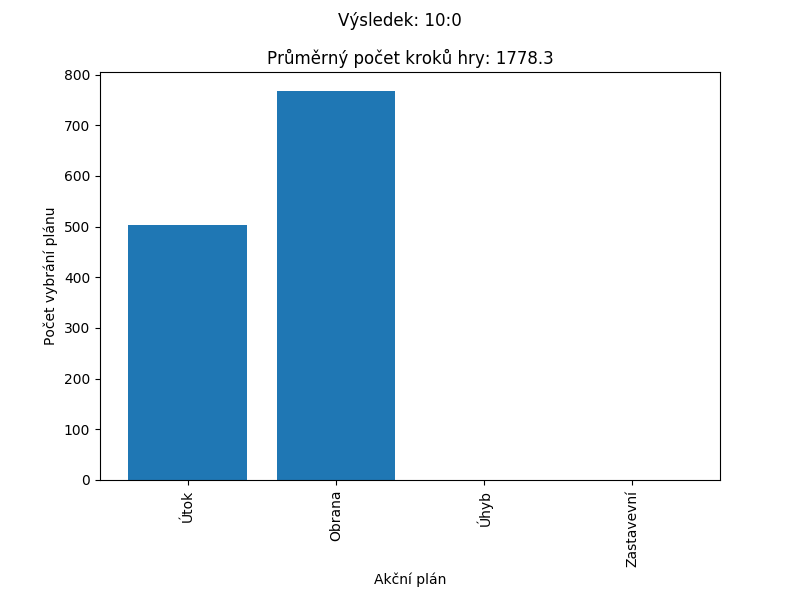
\includegraphics[width=125mm, height=100mm]{./Obrazky/Experiment02Results.png}
\caption{Výsledek experimentu 02}
\label{obr04:Výsledek experimentu 02}
\end{figure}










\begin{figure}[p]\centering
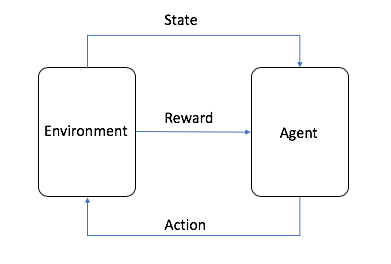
\includegraphics[width=140mm, height=140mm]{./agent_enviroment}
\caption{Herní cyklus}
\label{obr03:Nhust}
\end{figure}
